\subsection{Frequency-Domain Heterodyne detection}
\label{sec:heterodyne}
The primary goal of the frequency-domain DOT system is to measure the AC and phase components of the signal for each source detector pair. Two approaches are used to demodulate a high frequency RF signal: homodyne and heterodyne. Several homodyne systems have been developed for diffuse optical imaging \cite{Troy1996,Sevick-Muraca1997,Godavarty2003}, but here we describe the heterodyne approach.

Our system uses the optical heterodyne detection scheme wherein an input signal modulated at frequency, $f_{s}$, is nonlinearly mixed with a reference signal which is modulated at a frequency that is offset from $f_{s}$ by a small cross-correlation frequency, $f_{cc}$, such that the detection gain frequency $f_{d}=f_{s}+f_{cc}$. The amplitude and phase data is thus derived from a signal that is oscillating (and is measured) at the beat frequency, $f_{cc}$. In our system, modulations frequencies at $f_{s}$ and  $f_{d}$ are provided a pair of phase-locked frequency generators (Rohde and Schwarz, SMA100A). The lasers in the devices are amplitude modulated at $f_{s}=70\,{\rm MHz}$. Therefore, the light source intensity is given by (rewriting Eqn.~\ref{AC})

\begin{equation}
S_s({\bf r}_s,t) = S_{dc}({\bf r}_s) + S_{ac}({\bf r}_s)\cos(2\pi f_s t)
\end{equation}

where the frequency $f=\omega/2\pi$ and ${\bf r_s}$ is the spatial position of the source. When the light passes through our breast tank (i.e., through breast or Intralipid solution) the measured fluence rate $\Phi$ which has the form

\begin{equation}
\label{eqn:FDfluence}
\Phi({\bf r}_s,{\bf r}_d,t) = \Phi_{dc}({\bf r}_s,{\bf r}_d) + \Phi_{ac}({\bf r}_s,{\bf r}_d)\cos(2\pi f_s t + \phi)
\end{equation}

where $\Phi_{dc}$, $\Phi_{ac}$, and $\phi$ are the DC, AC amplitude factors and phase shifts, respectively, that are impressed onto the light fluence-rate as it traverses the medium from the the source position ${\bf r}_s$ to detector position ${\bf r}_d$. Of course, these are the factors that have information about the sample, and which are inverted by DOT in order to derive optical absorption and scattering coefficients and, ultimately, tissue optical properites. From here onwards, I will drop ${\bf r}_s$ and ${\bf r}_d$ and assume that the equations refer to light measured for a specific source-detector pair (i.e. a single pixel) to simplify the derivations below.

The detection gain response of the image intensifier is determined by Fig.~\ref{fig:iigain} which in tern is controlled by the cathode voltage DC offset level, and the input AC modulation voltage. The intensifier is modulated at $f_d$ in such a way as to gate the intensifier on and off and produce a time-dependant gain curve that serves as a signal sampling system. This gives us the AC and $\phi$ components of the signal. The scenario is as follows

The cathode DC is set by the intensifier controller and the AC modulation is derived from the second frequency generator (modulated at $70\,{\rm MHz}+1\,{\rm Hz}$). Typically, the cathode DC offset is set to $0.8\,\rm{V}$ and the amplitude of the AC modulation is set to $1.8\,\rm{V}$ (As an aside, this corresponds to frequency generator output setting of $-13\,\rm{dBm}$). The gain is "off" until the modulation causes the bias to run up and down the linear part of the gain curve at voltages below $-1\rm{V}$ as shown in Fig.~\ref{fig:iigain}. The overall effect is to produce a gated gain curve with frequency $f_d$ and with some finite width. This is a commonly used technique for gated detection and sampling. In our analysis, we approximate the gain function by a series of Dirac delta functions - a delta ``comb" in time with peans at $t=nT_d$ where $T_d = 1/f_{d}$. Practically, in our instrument this comb will have a finite width which will only change our derivations below proportionally.

\begin{figure}[h]
\begin{center}
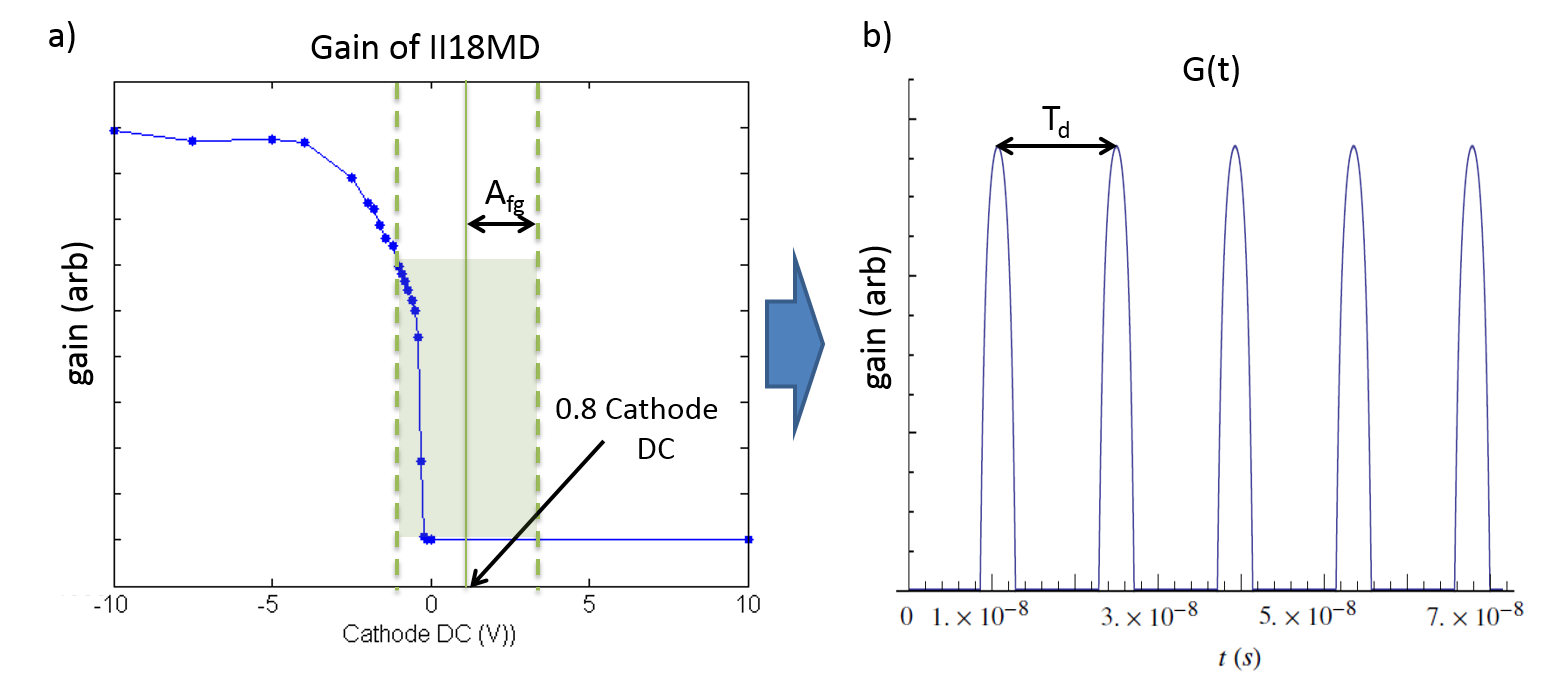
\includegraphics[width=14cm]{./figures/4_Gen3/iigain.png}
\caption{a) Measured gain response curve for the image intensifier for various cathode voltage values. Green solid line shows where the cathode DC value is set to $0.8\,\rm{V}$ Red curve shows the input AC voltage modulation from the frequency generator with an amplitude of $1.8\,\rm{V}$. b) Shows the modeled gain curve as a function of time produced from the curve in a). These curves can be treated as Dirac delta functions with a finite width.}
\label{fig:iigain}
\end{center}
\end{figure}
\noindent
If we model our detection system as a Dirac comb modulated at $70\,\rm{MHz} + 1\,\rm{Hz}$ the equation for our gain will be.
\begin{equation}
\label{eqn:diraccomb}
G(t)\equiv\sum_{n=-\infty}^{\infty} \delta(t - nT_d).
\end{equation}
\noindent
Where $T_d=1/f_d$ is the period of our gain modulation. Then the measured signal $M$ at the CCD is simply the product of Eqn.~\ref{eqn:FDfluence} and \ref{eqn:diraccomb} which is
\begin{align}
M(t)
&=\Phi(t)G(t) \notag \\
&=\left(\Phi_{dc} + \Phi_{ac} \cos(2 \pi f_s t+\phi)\right)\left( \sum_{n=-\infty}^{\infty}\delta(t-n T_d)\right)
\end{align}
\noindent
To help us solve this equation we rely on the convolution theorem which states that the multiplication in the time domain is equivalent to a convolution in the frequency domain. To use this theorem we need the Fourier transform of the fluence rate and the gain. The Fourier transform for the fluence rate is
\begin{align}
\label{eqn:srcFT}
\hat{\Phi}(f)
&=\int_{-\infty}^{\infty} \left(\Phi_{dc}+\Phi_{ac} \cos(2 \pi f_s t+\phi)\right) e^{- 2 \pi i f t} dt \notag \\
&=\Phi_{dc} \int_{-\infty}^{\infty} e^{- 2 \pi i f t} dt + \frac{\Phi_{ac}}{2} \int_{-\infty}^{\infty} \left( e^{i(2 \pi f_s t+\phi)} + e^{-i(2 \pi f_s t+\phi)}\right) e^{-2 \pi i f t} dt \notag \\
&=\Phi_{dc} \delta(f) + \frac{\Phi_{ac}}{2} \int_{-\infty}^{\infty} \left(e^{-2 \pi i(f-f_s)t+i\phi}+e^{-2 \pi i (f_s+f)t-i\phi}\right) dt \notag \\
&=\Phi_{dc} \delta(f) + \frac{\Phi_{ac}}{2} \left( \delta(f-f_s)e^{i\phi}+\delta(f+f_s)e^{-i\phi}\right)
\end{align}
And it is well known that the Fourier transform of a Dirac comb is
\begin{align}
\label{eqn:diracFT}
\hat{G}(f)
&=\frac{1}{T_d}\sum_{n=-\infty}^{\infty} \delta\left( f - \frac{n}{T_d}\right)
\end{align}
\noindent
Now the convolution of Eqn.~\ref{eqn:srcFT} and \ref{eqn:diracFT} is
\begin{align}
\label{eqn:Mconv}
\hat{M}(f)
&=\hat{\Phi}*\hat{G}\\
&=\int_{-\infty}^{\infty} \left[\Phi_{dc} \delta(f') + \frac{\Phi_{ac}}{2} \left( \delta(f'-f_s)e^{i\phi} + \delta(f'+f_s)e^{-i\phi}\right)\right] \hat{G}(f-f')df' \notag \\
&=\Phi_{dc} \int_{-\infty}^{\infty} \delta(f') C(f-f') df' + \\
& \qquad \frac{\Phi_{ac}}{2} \int_{-\infty}^{\infty} \left( \delta(f'-f_s)e^{i\phi}+\delta(f'+f_s)e^{-i\phi}\right) G(f-f') df' \notag \\
&=\Phi_{dc} G(f)+ \frac{\Phi_{ac}}{2}\left(G(f-f_s)e^{i\phi}+G(f+f_s)e^{-i\phi}\right)
\end{align}
Using the definition of the Dirac Comb in Eqn.~\ref{eqn:diraccomb}, Eqn.~\ref{eqn:Mconv} becomes
\begin{align}
\hat{M}(f)=\frac{\Phi_{dc}}{T_{d}} \sum_{n=-\infty}^{\infty} \left[\delta \left( f - \frac{n}{T_{d}}\right)+\frac{\Phi_{ac}}{2} \left(\delta \left(f-f_s-\frac{n}{T_{d}}\right)e^{i\phi} + \delta\left(f+f_s-\frac{n}{T_{d}}\right)e^{-i\phi}\right)\right]
\end{align}
Expanding the first term ($n=0$) we get
\begin{equation}
\hat{M}_0(f)=\frac{1}{T_{d}}\Big[\Phi_{dc}\delta(f)+\frac{\Phi_{ac}}{2}\Big( \delta(f-f_s)e^{i\phi}+\delta(f+f_s)e^{-i\phi}\Big)\Big]
\end{equation}
\noindent
For which the inverse Fourier transform is
\begin{equation}
M_0(t)=\mathcal{F}^{-1}\Big[\hat{M_0}(f)\Big] =\frac{1}{T_{d}}\Big(\Phi_{dc}+\Phi_{ac}\cos(2\pi f_st+\phi)\Big)
\end{equation}
\noindent
For $n=1$
\begin{align}
M_{1}(f)
&=\frac{1}{T_{d}}
\left[\Phi_{dc}\delta\left(f-\frac{1}{T_{d}}\right)+\frac{\Phi_{ac}}{2}\left(\delta\left( f-f_s-\frac{1}{T_{d}}\right)e^{i\phi}+\delta \left(f+f_s-\frac{1}{T_{d}}\right)e^{-i\phi}\right)\right] \notag\\
&=\frac{1}{T_{d}}\left[\Phi_{dc} \delta(f-f_s)+\frac{\Phi_{ac}}{2} \left(\delta(f-f_s-f_d)e^{i\phi}+\delta(f+f_s-f_d)e^{-i\phi}\right)\right]\notag\\
&=\frac{1}{T_{d}}\left[\Phi_{dc} \delta(f-f_s)+\frac{\Phi_{ac}}{2}\left(\delta(f-2f_s-f_{cc})e^{i\phi}+\delta(f-f_{cc})e^{-i\phi}\right)\right]
\end{align}
\noindent 
where I have used the subtitution $f_d=f_s+f_{cc}$ in the last step. The corresponding inverse Fourier transform is
\begin{align}
M_{1}(t)
&= \frac{1}{T_{d}} \int_{-\infty}^{\infty} \Big[\Phi_{dc}\delta(f-f_s) \\
& \qquad + \frac{\Phi_{ac}}{2} \left(\delta(f-2f_s-f_{cc})e^{i\phi}+\delta(f-f_{cc})e^{-i\phi}\right)\Big] e^{2 \pi i f t}df
\end{align}
 Similarly for $n=-1$
\begin{align}
M_{n=-1}(t)
&= \frac{1}{T_{d}} \int_{-\infty}^{\infty} \Big[\Phi_{dc}\delta(f+f_s) \\
& \qquad + \frac{\Phi_{ac}}{2} \left(\delta(f+f_{cc})e^{i\phi}+\delta(f+2f_s+f_{cc})e^{-i\phi}\right)\Big] e^{2 \pi i f t}df
\end{align}
Combining $M_1$ and $M_{-1}$ gives us
\begin{align}
M_{\pm 1}(t)
&= \frac{\Phi_{dc}}{T_{d}} \int_{-\infty}^{\infty} \Big(\delta(f-f_s)+\delta(f+f_s)\Big)e^{2 \pi i f t}df \notag \\
& \qquad + \frac{\Phi_{ac}}{2T_{d}} \int_{-\infty}^{\infty} \Big(\delta(f-2f_s-f_{cc})e^{i\phi} + \delta(f+2f_s+f_{cc})e^{-i\phi}\Big) e^{2 \pi i f t}df \notag \\
& \qquad + \frac{\Phi_{ac}}{2T_{d}} \int_{-\infty}^{\infty} \Big(\delta(f-f_{cc})e^{i\phi} + \delta(f+f_{cc})e^{-i\phi}\Big) e^{2 \pi i f t}df \notag\\
&=\frac{\Phi_{dc}}{2T_{d}} \cos(2\pi f_s t)+ \frac{\Phi_{ac}}{4T_{d}} \cos(2\pi(2f_s+f_{cc})+\phi) + \frac{\Phi_{ac}}{4T_{d} }\cos(2\pi(f_{cc})+\phi)
\end{align}
\noindent
One can then write down the full series for $M(t)$ as
\begin{align}
M(t)
&= \frac{1}{T_{d}}\Big(\Phi_{dc}+\Phi_{ac}\cos(2\pi f_st+\phi)\Big) & (M_0\,{\rm term}) \notag\\
& + \frac{\Phi_{dc}}{2T_{d}} \cos(2\pi f_s t)+ \frac{\Phi_{ac}}{4T_{d}} \cos(2\pi(2f_s+f_{cc})+\phi) + \underline{\frac{\Phi_{ac}}{4T_{d} }\cos(2\pi(f_{cc})+\phi)} & (M_{\pm 1}\,{\rm term}) \notag\\
& + \frac{1}{T_d}\sum_{n=2}^{\infty}\Big[\frac{\Phi_{dc}}{2} \cos(2 \pi n f_st) + \frac{\Phi_{ac}}{4}\Big(\cos(2 \pi(f_s-n f_d)t+\phi) & (n\geq 1\,{\rm terms}) \notag\\
& \qquad + \cos(2 \pi(f_s+n f_d)t+\phi)\Big)\Big] &
\end{align}
This is the equation for the measured light at our CCD for a given pixel. In our experiment however, the response time of the detection is limited by our CCD exposure time which is $\sim 100\,{\rm ms}$ or the frame rate which is $10 \rm{Hz}$. Any term with a modulation frequency greater than $10\,\rm{Hz}$ (and certainly any term in the MHz range) will become a constant. Since we are only concerned with measuring the $\Phi_{ac}$ and $\phi$, then the terms we are interested is given by the underlined term.
\begin{align}
\label{eqn:heterodyneresult}
M(t)
&= \frac{\Phi_{dc}}{T_d} + \underline{\frac{\Phi_{ac}}{4T_{d}}\cos(2\pi f_{cc} t+\phi)} + \big(\rm{higher\,freq.\,terms}\big) \notag\\
&\propto \underline{\Phi_{ac}\cos(2\pi f_{cc} t+\phi)} + \big(\rm{a\,constant}\big)
\end{align}